\documentclass[a4paper,12pt]{article}
\usepackage{tikz}
\usetikzlibrary{positioning, shapes.geometric, arrows.meta}
\usepackage{tabularx} % For tables with text wrapping
\usepackage{booktabs} % For better tables
\usepackage{hyperref}
\usepackage[a4paper, left=2cm, right=4cm, top=2.5cm, bottom=2.5cm]{geometry}
\usepackage{ragged2e} % for \RaggedRight in tables
\usepackage{array} % for >{\raggedright\arraybackslash}p{} in tables
\usepackage{float}

\title{Design and Normalization Database on SuperMarket Aisle Management}
\author{Fadhla Mohamed Mutua - SM3201434}
\date{\today}

\begin{document}
\maketitle

\begin{abstract}
This report presents the conceptual and logical design of a supermarket aisle management database. The system manages supermarkets, aisles, items, producers, distances, and error logging for items. Explained are the SQL operations to be used (see accompanying code), Entity-Relationship (ER) diagrams, redundancy and normalization steps up to Third Normal Form (3NF).
\end{abstract}

\newpage
\tableofcontents
\newpage

\section{Introduction}
This report is on a database system that supports supermarkets, and, producers by logging errors generated by automated triggers.

\section*{2. SQL Operations Overview}

This section outlines all the core SQL operations implemented in the database system, explaining their roles and how they support the domain logic of aisle management and compliance.

\subsection*{2.1 Creation of Tables}

\textbf{Operation: Schema Definition and Initialization}

The first set of operations defines the relational structure and schema of the database. Tables such as \texttt{SuperMarket}, \texttt{Aisle}, \texttt{Item}, \texttt{Producer}, \texttt{Distance}, \texttt{Contain}, \texttt{Manufactured\_By}, \texttt{ErrorMessages}, and \texttt{ItemLogErrors} are created using \texttt{CREATE TABLE}. These statements specify primary and foreign keys, data types, and constraints, establishing the foundation for data storage.

\subsection*{2.2 Triggers}

\textbf{Trigger: \texttt{trg\_check\_Item\_Aisle\_count}}

This \texttt{BEFORE INSERT} trigger ensures that an item is not placed in multiple aisles within the same supermarket. If violated, it raises an SQL exception. This guarantees one-to-one mapping of item to aisle per supermarket.

\textbf{Trigger: \texttt{trg\_log\_item\_wrong\_aisle}}

This \texttt{AFTER INSERT} trigger validates whether the item is placed in a logically correct aisle using a function. If non-compliant, it logs the violation via an error ID, using standardized messages and timestamping.

\textbf{Trigger: \texttt{ReturnItem}}

Monitors inserted items for expiration. If an item is expired, it checks if the distance to the producer is within a threshold or if the item is non-perishable. It then logs whether the item should be returned or thrown away.

\subsection*{2.3 Views}

\textbf{View: \texttt{FullItemDetails}} — Comprehensive joined result showing each item, its aisle, supermarket, and producer.

\textbf{View: \texttt{ItemWithProducers}} — Displays item and associated producer information.

\textbf{View: \texttt{ProducerSuperMarketDistance}} — Maps distances between producers and supermarkets.

\textbf{View: \texttt{WhereToStore}} — Matches storage types of items with aisle names for placement validation.

\textbf{View: \texttt{ItemErrorDetails}} — Provides detailed logs of item errors including messages and discard flags.

\subsection*{2.4 Stored Functions}

\textbf{Function: \texttt{fn\_validate\_aisle\_compliance}}

Enforces domain rules for aisle placement. Returns a human-readable error if non-compliant, otherwise \texttt{NULL}.

\textbf{Function: \texttt{fn\_insert\_into\_error\_message}}

Inserts a new message into \texttt{ErrorMessages} table if it doesn’t exist and returns the \texttt{ErrorID}.

\textbf{Function: \texttt{fn\_suggest\_correct\_aisle}}

Suggests the most appropriate \texttt{AisleID} for an item in a specific supermarket based on category and storage.

\subsection*{2.5 Stored Procedures}

\textbf{Procedure: \texttt{pr\_insert\_item\_log}} — Inserts item error logs with timestamp and error info.

\textbf{Procedure: \texttt{AddItemToAisle}} — Adds an item to an aisle, verifying that the aisle belongs to the specified supermarket.

\textbf{Procedure: \texttt{RemoveItemFromSuperMarket}} — Deletes an item from all aisles in a supermarket.

\textbf{Procedure: \texttt{LogItemError}} — Logs a manual item error using message and item details.

\textbf{Procedure: \texttt{CleanExpiredItems}} — Deletes expired and perishable items from the \texttt{Contain} table.

\textbf{Procedure: \texttt{CheckItemCompliance}} — Checks compliance and optionally suggests correct placement.

\textbf{Procedure: \texttt{sp\_check\_item\_placement}} — Iterates through items, validates placement, and logs non-compliance.

\textbf{Procedure: \texttt{sp\_expiration\_check}} — Logs expiration-related issues including producer and discard status.

\subsection*{2.6 Scheduled Events}

\textbf{Event: \texttt{ev\_daily\_item\_placement\_check}} — Daily trigger to run \texttt{sp\_check\_item\_placement}.

\textbf{Event: \texttt{ev\_daily\_expiration\_and\_cleanup}} — Daily cleanup of expired items and logging of expiration status.

\textbf{Event: \texttt{ev\_daily\_expiration\_process}} — Wrapper event managing expiration and cleanup automation.

\subsection*{2.7 Queries}

\textbf{Query: Historical Error Analysis}

\begin{verbatim}
SELECT
    em.ErrorMessage,
    i.ItemName, i.ItemStorageType,
    a.AisleID, a.AisleName AS IncorrectAisle,
    le.LogTime,
    le.ToBeThrown
FROM ItemLogErrors le
JOIN Item i ON le.ItemID = i.ItemID
JOIN Aisle a ON le.AisleID = a.AisleID
LEFT JOIN ErrorMessages em ON le.ErrorID = em.ErrorID
ORDER BY le.LogTime DESC;
\end{verbatim}

Provides a full log of item placement or expiration violations with contextual information.

\section{Conceptual Schema}

\subsection{Conceptual Schema Table}

\begin{table}[H]
\centering
\begin{tabularx}{\textwidth}{@{} l >{\RaggedRight\arraybackslash}X @{}}
\toprule
\textbf{Entities and Relationship} & \textbf{Cardinality (Relational)} \\ \midrule
Producer — Distance — SuperMarket & 0:N : 1:N \\
SuperMarket — Has\_Aisle — Aisle & 1:N : 1:1 \\
Aisle — Contains — Item & 1:N : 1:1 \\
Producer — Manufactured\_By — Item & 0:N : 1:1 \\
ItemLogErrors — Logs\_Item — Item & 1:1 : 1:N \\
ItemLogErrors — Logs\_Aisle — Aisle & 1:1 : 1:N \\
ItemLogErrors — Logs\_ErrorMessage — ErrorMessage & 1:1 : 1:N \\
\bottomrule
\end{tabularx}
\caption{Conceptual Schema Relations with Precise Cardinalities}
\label{tab:conceptual-schema}
\end{table}

\begin{table}[H]
\centering
\begin{tabularx}{\textwidth}{@{} l >{\RaggedRight\arraybackslash}X @{}}
\toprule
\textbf{Relationship} & \textbf{Description} \\ \midrule
Distance & Connects producers to supermarkets with distance information, useful for calculating transportation and supply chain logistics. \\ 
Has\_Aisle & Associates aisles to supermarkets, indicating the layout structure within each store. \\ 
Contains & Represents items stored within aisles, linking inventory to location. \\ 
Manufactured\_By & Links items to their producers, allowing traceability of product origins. \\ 
Logs\_Item & Logs errors related to specific items, facilitating error tracking and auditing. \\ 
Logs\_Aisle & Logs errors associated with specific aisles, aiding in pinpointing storage issues. \\ 
Logs\_ErrorMessage & Associates error logs with standardized error messages, enabling consistent error reporting. \\ 
\bottomrule
\end{tabularx}
\caption{Conceptual Schema Relationships and Their Description}
\label{tab:relationship-descriptions}
\end{table}

\subsection{Entity-Relationship Diagram}
\newpage

\begin{figure}[H]
\hspace*{-2cm} % shift left by 2cm
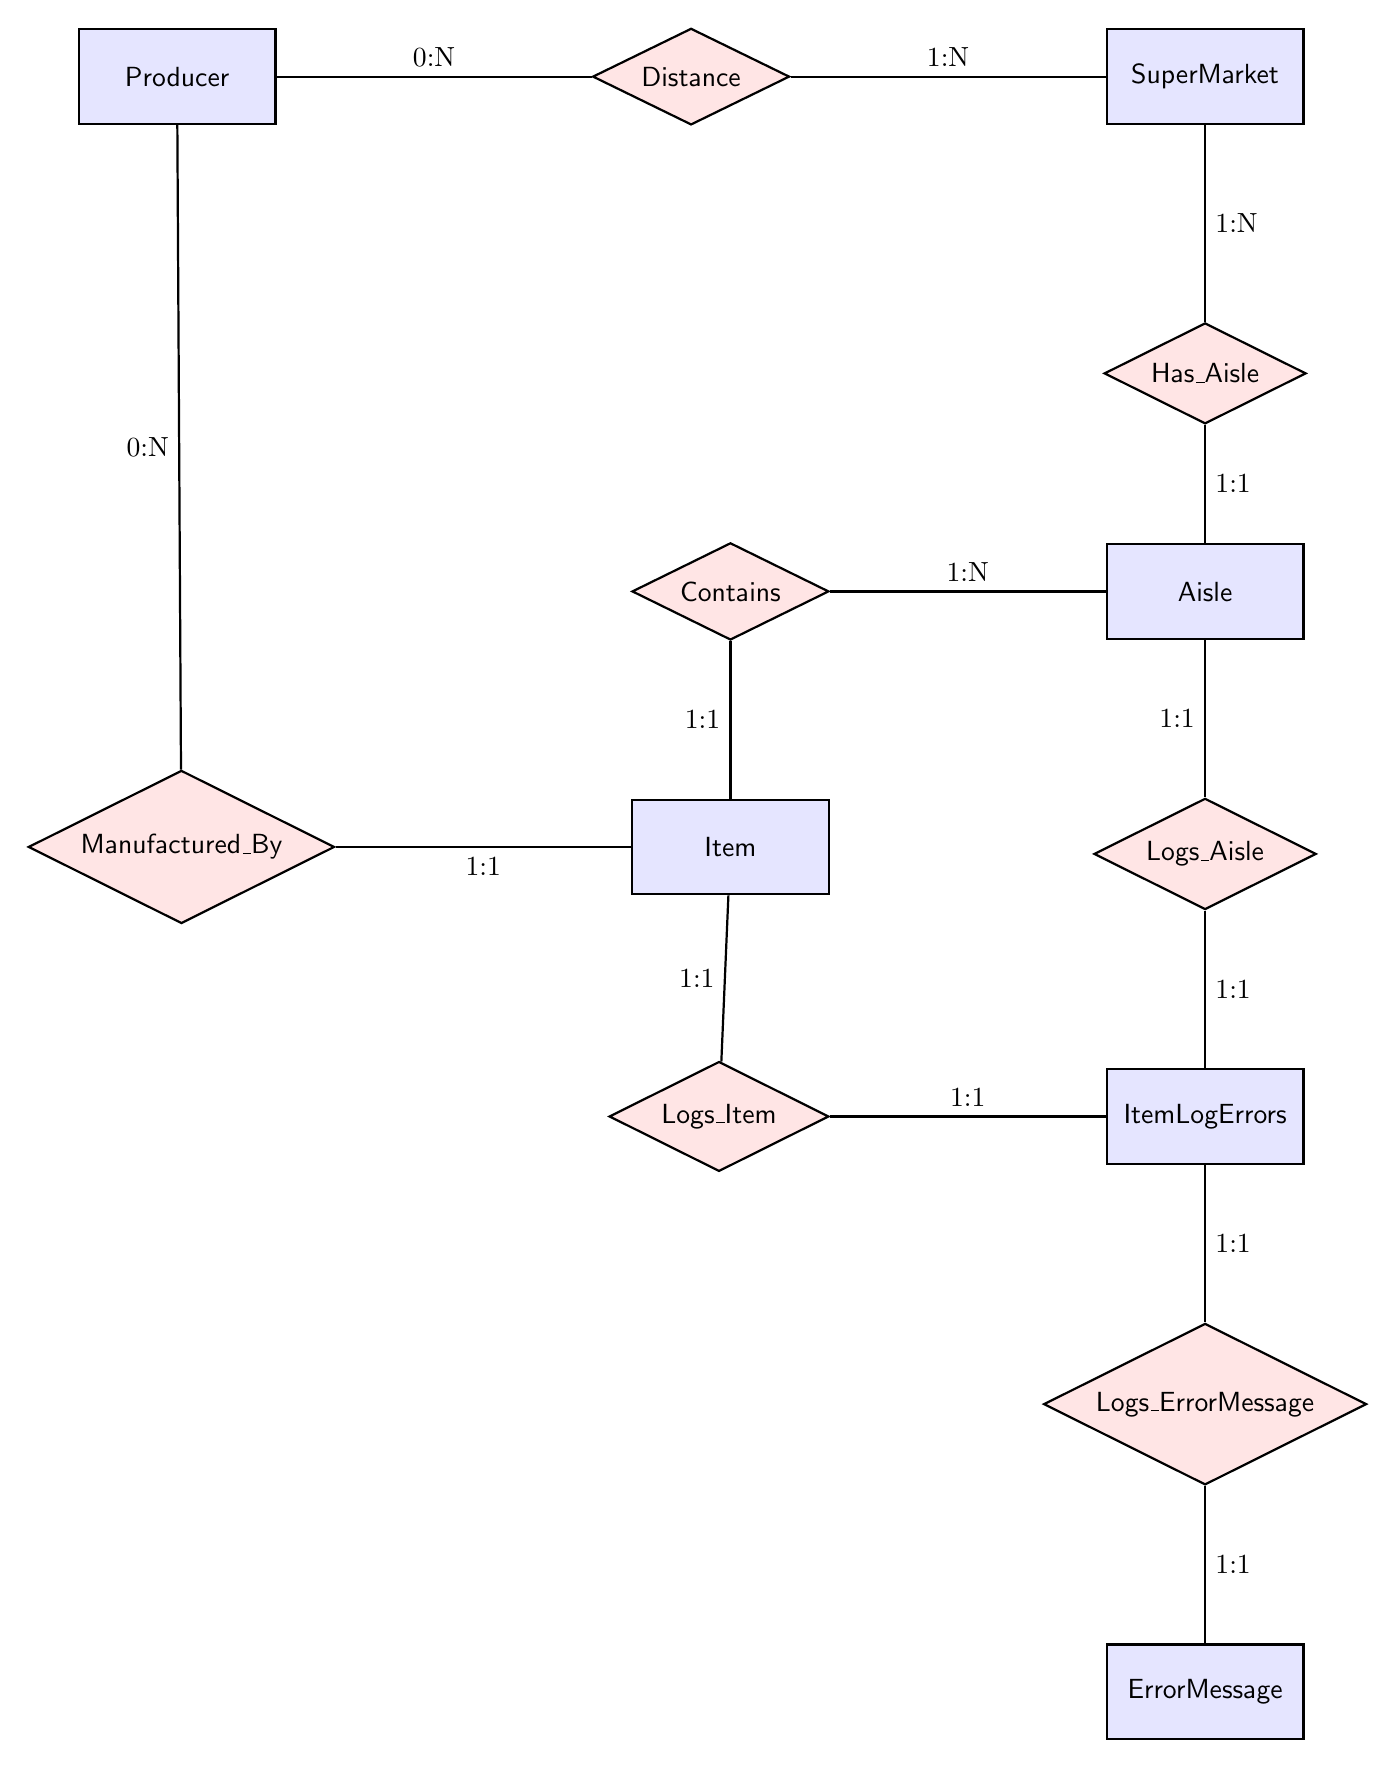
\begin{tikzpicture}[
  entity/.style={rectangle, draw=black, thick, minimum width=2.5cm, minimum height=1.2cm, fill=blue!10, font=\sffamily},
  relationship/.style={diamond, draw=black, thick, aspect=2, minimum width=2.5cm, minimum height=1.2cm, fill=red!10, font=\sffamily},
  line/.style={thick},
  every label/.style={font=\footnotesize},
  node distance=2cm and 3cm
]

% Entities and relationships placed relatively
\node[entity] (P) {Producer};
\node[relationship, right=4cm of P] (D) {Distance};
\node[entity, right=4cm of D] (S) {SuperMarket};

\node[relationship, below=2.5cm of S] (H) {Has\_Aisle};
\node[entity, below=1.5cm of H] (A) {Aisle};

\node[relationship, left=3.5cm of A] (C) {Contains};
\node[entity, below=2cm of C] (I) {Item};

\node[relationship, left=3.75cm of I] (M) {Manufactured\_By};

\node[relationship, below=2cm of A] (IL_A) {Logs\_Aisle};
\node[entity, below=2cm of IL_A] (Ie) {ItemLogErrors};
\node[relationship, left=3.5cm of Ie] (IL_I) {Logs\_Item};
\node[relationship, below=2cm of Ie] (IL_E) {Logs\_ErrorMessage};
\node[entity, below=2cm of IL_E] (E) {ErrorMessage};

% Draw edges with cardinalities
\draw[line] (P) -- node[above] {0:N} (D);
\draw[line] (D) -- node[above] {1:N} (S);

\draw[line] (S) -- node[right] {1:N} (H);
\draw[line] (H) -- node[right] {1:1} (A);

\draw[line] (A) -- node[above] {1:N} (C);
\draw[line] (C) -- node[left] {1:1} (I);

\draw[line] (P) -- node[left] {0:N} (M);
\draw[line] (M) -- node[below] {1:1} (I);

\draw[line] (Ie) -- node[above] {1:1} (IL_I);
\draw[line] (IL_I) -- node[left] {1:1} (I);

\draw[line] (Ie) -- node[right] {1:1} (IL_A);
\draw[line] (IL_A) -- node[left] {1:1} (A);

\draw[line] (Ie) -- node[right] {1:1} (IL_E);
\draw[line] (IL_E) -- node[right] {1:1} (E);

\end{tikzpicture}
\caption{Entity-Relationship Diagram for Aisle Management}
\label{fig:er-diagram}
\end{figure}

\newpage
\subsection{Redundancy Analysis}

\begin{itemize}
    \item \textbf{ItemLogErrors} has multiple binary relationships with \texttt{Item}, \texttt{Aisle}, and \texttt{ErrorMessage}.
    \item This could be replaced by a ternary relationship directly linking \texttt{ItemLogErrors} with \texttt{Item}, \texttt{Aisle}, and \texttt{ErrorMessage}.
    \item Since \texttt{ItemLogErrors} is trigger-generated, keeping the separate relationships together eases querying.
    \item No redundant entities or relationships for \texttt{Producer}, \texttt{SuperMarket}, \texttt{Aisle}, \texttt{Item}, or \texttt{Distance}.
\end{itemize}

\newpage
\section{Logical Schema}

\begin{table}[H]
\centering
\begin{tabularx}{\textwidth}{@{} l @{\hspace{1.5cm}} >{\RaggedRight\arraybackslash}X @{\hspace{1.5cm}} p{2.5cm} @{\hspace{1cm}} p{2.5cm} @{}}
\toprule
\textbf{Table} & \textbf{Attributes} & \textbf{PK} & \textbf{FK} \\ 
\midrule
Producer & ProducerID, ProducerName, ProducerLocation & \underline{ProducerID} & - \\ \hline
SuperMarket & SuperMarketID, SuperMarketName, SuperMarketLocation & \underline{SuperMarketID} & - \\ \hline
Aisle & AisleID, SuperMarketID, AisleName & \underline{AisleID} & SuperMarketID \\ \hline
Item & ItemID, ItemName, ItemCategory, ItemStorageType, ItemPerishable, ItemExpirationDate & \underline{ItemID} & - \\ \hline
Manufactured\_By & ItemID, ProducerID & \underline{ItemID} & ProducerID \\ \hline
Distance & ProducerID, SuperMarketID, Distance & \underline{ProducerID}, \underline{SuperMarketID} & ProducerID, SuperMarketID \\ \hline
Contain & AisleID, ItemID & \underline{AisleID}, \underline{ItemID} & AisleID, ItemID \\ \hline
ItemLogErrors & ErrorLogID, ItemID, AisleID, ErrorID, LogTime, ToBeThrown & \underline{ErrorLogID} & ItemID, AisleID, ErrorID \\ \hline
ErrorMessage & ErrorID, ErrorMessage & \underline{ErrorID} & - \\
\bottomrule
\end{tabularx}
\caption{Logical Schema Tables with Underlined Primary Keys}
\end{table}

\newpage
\section{Normalization}

\subsection{First Normal Form (1NF)}
\begin{itemize}
    \item All attributes are atomic and indivisible.
    \item No repeating arrays exist as ErrorMessage message is a String.
\end{itemize}

\subsection{Second Normal Form (2NF)}
\begin{itemize}
    \item No partial dependency exists on composite keys.
\end{itemize}

\subsection{Third Normal Form (3NF)}
\begin{itemize}
    \item No transitive dependencies are present.
    \item All non-key attributes depend only on the primary key.
    \item Example: In \texttt{Item}, all attributes (category, perishable flag, expiration) depend only on \texttt{ItemID}.
    \item No derived or calculated fields are stored, avoiding redundancy.
\end{itemize}

\begin{table}[H]
\centering
\begin{tabularx}{\textwidth}{@{} l >{\RaggedRight\arraybackslash}X @{}}
\toprule
\textbf{Entities and Relationship} & \textbf{Cardinality (can/(or) must : quantity \quad : \quad can/(or) must : quantity)} \\ \midrule
Producer — Distance — SuperMarket & 0:N : 1:N \\
SuperMarket — Has\_Aisle — Aisle & 1:N : 1:1 \\
Aisle — Contains — Item & 1:N : 1:1 \\
Producer — Manufactured\_By — Item & 0:N : 1:1 \\
ItemLogErrors — Logs\_Item — Item & 1:1 : 1:N \\
ItemLogErrors — Logs\_Aisle — Aisle & 1:1 : 1:N \\
ItemLogErrors — Logs\_ErrorMessage — ErrorMessage & 1:1 : 1:N \\
\bottomrule
\end{tabularx}
\caption{Normalized Conceptual Schema with precise cardinalities}
\end{table}

\begin{table}[H]
\centering
\begin{tabularx}{\textwidth}{@{} l >{\RaggedRight\arraybackslash}X @{\hspace{1cm}} p{2.2cm} @{\hspace{0.8cm}} p{2.2cm} @{}}
\toprule
\textbf{Table} & \textbf{Attributes} & \textbf{PK} & \textbf{FK} \\ 
\midrule
Producer & ProducerID, ProducerName, ProducerLocation & \underline{ProducerID} & - \\ \hline
SuperMarket & SuperMarketID, SuperMarketName, SuperMarketLocation & \underline{SuperMarketID} & - \\ \hline
Aisle & AisleID, SuperMarketID, AisleName & \underline{AisleID} & SuperMarketID \\ \hline
Item & ItemID, ItemName, ItemCategory, ItemStorageType, ItemPerishable, ItemExpirationDate & \underline{ItemID} & - \\ \hline
Manufactured\_By & ItemID, ProducerID & \underline{ItemID} & ProducerID \\ \hline
Distance & ProducerID, SuperMarketID, Distance & (\underline{ProducerID}, \underline{SuperMarketID}) & ProducerID, SuperMarketID \\ \hline
Contain & AisleID, ItemID & (\underline{AisleID}, \underline{ItemID}) & AisleID, ItemID \\ \hline
ItemLogErrors & ErrorLogID, ItemID, AisleID, ErrorID, LogTime, ToBeThrown & \underline{ErrorLogID} & temID, AisleID, ErrorID \\ \hline
ErrorMessage & ErrorID, ErrorMessage & \underline{ErrorID} & - \\
\bottomrule
\end{tabularx}
\caption{Normalized Logical Schema}
\end{table}

\section{Conclusion}

The normalization process confirms the schema adheres to 3NF, supporting automated error tracking without introducing redundancy.

\end{document}
